% ============================================================================
% METODIKA
% Podľa metodických pokynov FZ TnUAD
% Písané v 1. osobe množného čísla, minulý čas (autorský plurál)
% ============================================================================

\chapter{Cieľ práce a metodológia}

Praktická časť diplomovej práce je zameraná na overenie účinnosti navrhnutej terapie. V~tejto kapitole definujeme hlavný a~čiastkové ciele práce, stanovujeme hypotézy a~charakterizujeme výskumný súbor. Ďalej popisujeme metodiku zberu dát a~postup spracovania získaných výsledkov.

\section{Cieľ práce}

Cieľom diplomovej práce bolo na základe dostupnej literatúry a~vlastného výskumu posúdiť účinnosť fyzioterapie pri liečbe pacientov s~reumatoidnou artritídou.

\textbf{Hlavný cieľ:}
Zistiť, ako kombinovaná liečba interferenčnými prúdmi a~kinezioterapiou ovplyvňuje intenzitu bolesti, rozsah pohybu a~subjektívne hodnotenie kvality života pacientov s~reumatoidnou artritídou.

\textbf{Čiastkové ciele:}
\begin{enumerate}
    \item Porovnať účinnosť kombinovanej terapie (IFP + kinezioterapia) a~samotnej kinezioterapie na intenzitu bolesti.
    \item Analyzovať vplyv kombinovanej terapie na rozsah pohybu v~postihnutých kĺboch.
    \item Zhodnotiť subjektívne vnímanie kvality života pacientov pred a~po terapii.
    \item Porovnať výsledky experimentálnej a~kontrolnej skupiny.
\end{enumerate}

\section{Hypotézy}

Na základe stanovených cieľov sme formulovali nasledujúce hypotézy:

\textbf{H1:} Predpokladáme, že pacienti s~reumatoidnou artritídou, ktorí absolvujú terapiu interferenčnými prúdmi v~kombinácii s~kinezioterapiou, uvádzajú nižšiu intenzitu bolesti než pacienti liečení len kinezioterapiou.

\textbf{H2:} Predpokladáme, že kombinácia interferenčných prúdov a~kinezioterapie má väčší pozitívny vplyv na rozsah pohybu v~postihnutých kĺboch ako samotná kinezioterapia.

\textbf{H3:} Predpokladáme, že pacienti liečení kombinovanou terapiou subjektívne hodnotia kvalitu svojho života pozitívnejšie ako pacienti v~skupine bez elektroterapie.


\section{Charakteristika výskumného súboru}

Výskumný súbor tvorilo 100 pacientov s~potvrdenou diagnózou reumatoidnej artritídy. Podmienkou zaradenia do štúdie bola lekárom potvrdená diagnóza RA. Pacientov sme rozdelili do dvoch skupín po 50 jedincov. Experimentálnu skupinu tvorilo 50 pacientov absolvujúcich kombinovanú liečbu interferenčným prúdom a~kinezioterapiou. Kontrolnú skupinu tvorilo 50 pacientov podstupujúcich iba kinezioterapiu.

Graf zobrazuje rozdelenie mužov a~žien v~skupine s~kombinovanou liečbou aj v~skupine s~izolovanou kinezioterapiou.

\begin{figure}[H]
    \centering
    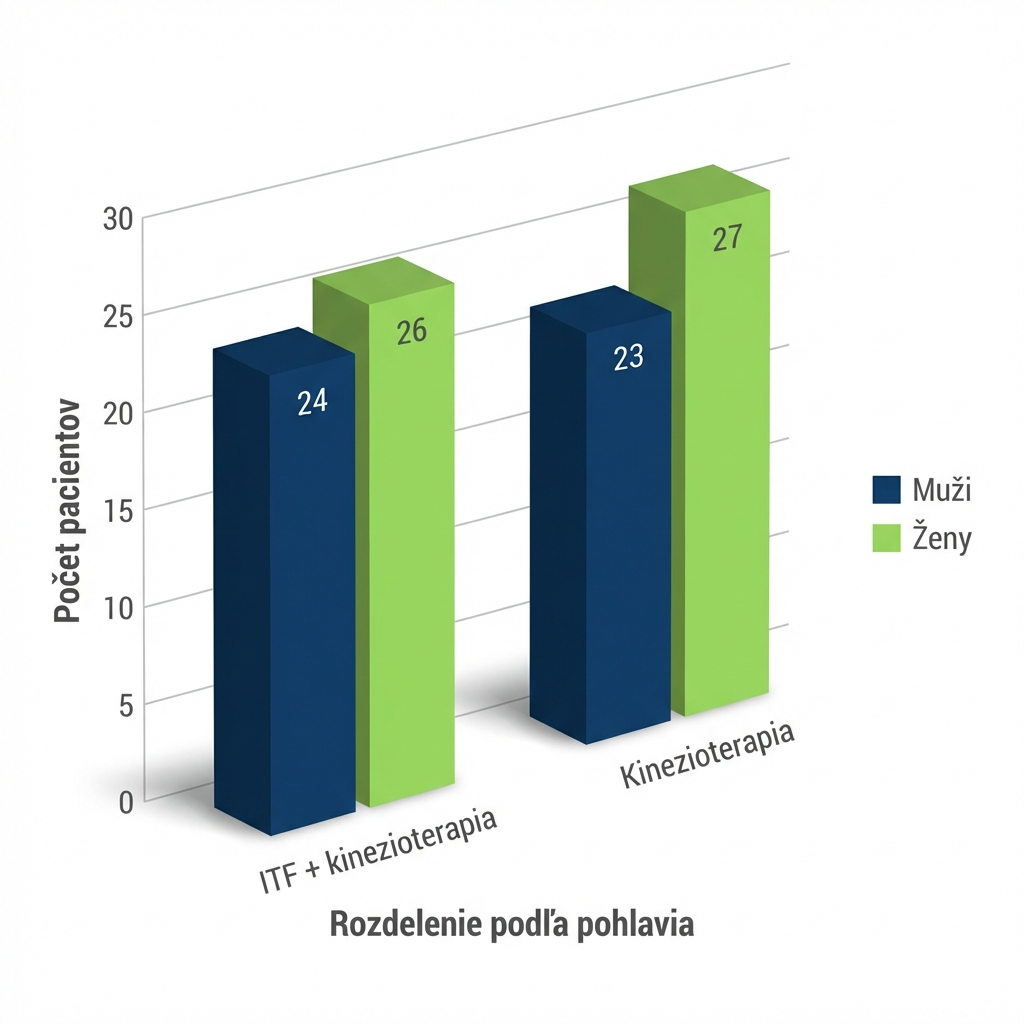
\includegraphics[width=0.8\textwidth]{obrazky/graf_zastupenie_pohlavie.png}
    \caption*{Graf 1 Počet mužov a~žien pre jednotlivé skupiny}
    \addcontentsline{lof}{figure}{Graf 1 Počet mužov a~žien pre jednotlivé skupiny}
    \label{fig:zastupenie_pohlavie}
\end{figure}

Skupinu s~kombinovanou liečbou tvorilo 24 mužov a~26 žien, pričom kontrolná skupina zahŕňala 23 mužov a~27 žien. Z~hľadiska rozloženia pohlavia možno konštatovať, že obe skupiny boli približne vyvážené.

Okrem základného rozdelenia podľa pohlavia sme sa zamerali aj na analýzu pracovného zaťaženia pacientov, keďže typ zamestnania môže významne ovplyvňovať mieru záťaže pohybového aparátu. V nasledujúcom grafe (Graf 2) je znázornená štruktúra súboru z hľadiska typu vykonávanej práce.

\begin{figure}[H]
    \centering
    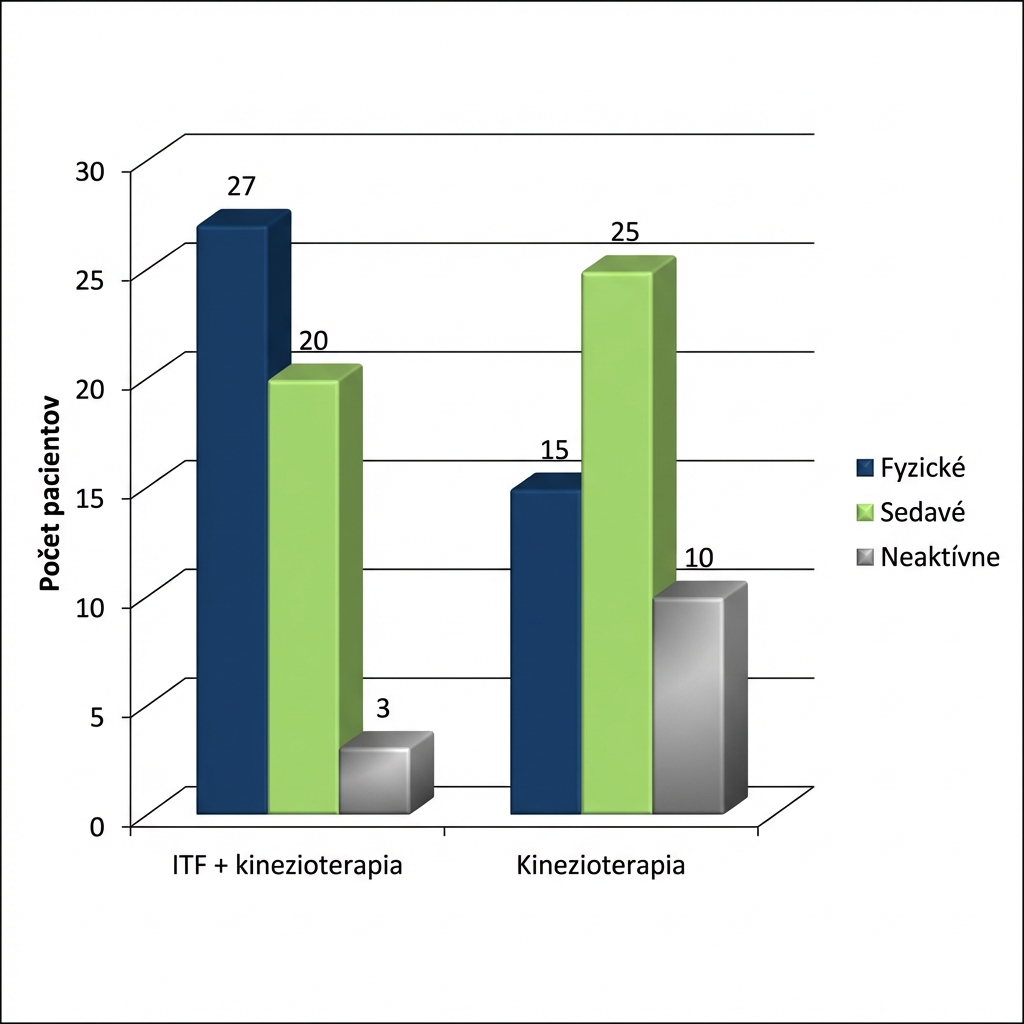
\includegraphics[width=0.8\textwidth]{obrazky/graf_zamestnanie.png}
    \caption*{Graf 2 Rozdelenie pacientov podľa typu zamestnania}
    \addcontentsline{lof}{figure}{Graf 2 Rozdelenie pacientov podľa typu zamestnania}
    \label{fig:zamestnanie}
\end{figure}

V~skupine s~kombinovanou terapiou (ITF + kinezioterapia) prevažovali pacienti s~manuálnym, resp. fyzickým zaťažením (n=27), za ktorými nasledovali pacienti so sedavým zamestnaním (n=20) a~najmenšiu časť tvorili neaktívni pacienti (n=3). Naopak, v~kontrolnej skupine (kinezioterapia) bolo zaznamenané vyššie zastúpenie pacientov so sedavým, resp. duševným zamestnaním (n=25), fyzicky pracujúcich bolo 15 a~skupinu neaktívnych pacientov (dôchodcovia alebo nezamestnaní) tvorilo 10 respondentov.

Súčasťou charakteristiky výskumného súboru bolo aj sledovanie základných demografických a antropometrických parametrov, ako sú vek, telesná výška a hmotnosť. Tieto údaje nám umožnili posúdiť homogenitu oboch skupín. Ako vyplýva z~údajov v~Tabuľke 1 a Tabuľke 2, obe skupiny vykazovali porovnateľné priemerné hodnoty sledovaných premenných, čo svedčí o~vysokej miere vyrovnanosti výskumnej vzorky. Táto podobnosť je dôležitá pre objektivitu porovnania terapeutických výsledkov.

\begin{table}[H]
\centering
\caption*{Tabuľka 1 Demografické údaje pacientov v skupine ITF + kinezioterapia}
\addcontentsline{lot}{table}{Tabuľka 1 Demografické údaje pacientov v skupine ITF + kinezioterapia}
\begin{tabular}{|l|c|c|c|c|c|c|}
\hline
\textbf{Pacienti} & \textbf{n} & \textbf{$\bar{x}$} & \textbf{sd} & \textbf{x$_m$} & \textbf{min.} & \textbf{max.} \\ \hline
Vek & 50 & 52,76 & 5,66 & 54,5 & 41 & 60 \\ \hline
Výška & 50 & 175,04 & 9,87 & 175,5 & 159 & 193 \\ \hline
Hmotnosť & 50 & 77,84 & 12,15 & 77,5 & 60 & 101 \\ \hline
\end{tabular}
\\
\footnotesize{Legenda: n~-- počet pacientov, $\bar{x}$~-- aritmetický priemer, sd~-- smerodajná odchýlka, $x_m$~-- medián, min.~-- minimálna hodnota, max.~-- maximálna hodnota}
\vspace{0.5em}
\newline
Skupina ITF + kinezioterapia vykazovala priemerný vek 52,76$\pm$5,66 roka, pričom priemerná telesná výška dosahovala 175,04$\pm$9,87 cm a hmotnosť 77,84$\pm$12,15 kg.
\label{tab:demografia_itf}
\end{table}

\begin{table}[H]
\centering
\caption*{Tabuľka 2 Demografické údaje pacientov v skupine Kinezioterapia}
\addcontentsline{lot}{table}{Tabuľka 2 Demografické údaje pacientov v skupine Kinezioterapia}
\begin{tabular}{|l|c|c|c|c|c|c|}
\hline
\textbf{Pacienti} & \textbf{n} & \textbf{$\bar{x}$} & \textbf{sd} & \textbf{x$_m$} & \textbf{min.} & \textbf{max.} \\ \hline
Vek & 50 & 51,62 & 6,18 & 52,5 & 40 & 60 \\ \hline
Výška & 50 & 173,04 & 10,23 & 174 & 157 & 190 \\ \hline
Hmotnosť & 50 & 74,22 & 11,06 & 74,0 & 57 & 96 \\ \hline
\end{tabular}
\\
\footnotesize{Legenda: n~-- počet pacientov, $\bar{x}$~-- aritmetický priemer, sd~-- smerodajná odchýlka, $x_m$~-- medián, min.~-- minimálna hodnota, max.~-- maximálna hodnota}
\vspace{0.5em}
\newline
V skupine liečenej samostatnou kinezioterapiou bol priemerný vek pacientov 51,62$\pm$6,18 roka. Priemerná výška týchto pacientov bola 173,04$\pm$10,23 cm a ich priemerná hmotnosť predstavovala 74,22$\pm$11,06 kg.
\label{tab:demografia_kin}
\end{table}





\clearpage
\clearpage
\section{Metodika výskumu}

Pre potreby nášho prieskumu sme zvolili metodologický postup kombinujúci subjektívne dotazníkové hodnotenie s~objektívnym meraním fyzických parametrov. Celý proces zberu údajov sa realizoval v~prostredí neštátneho zdravotníckeho zariadenia, pričom časový rámec bol stanovený od augusta 2025 do februára 2026. Probandi zapojení do štúdie absolvovali kompletný rehabilitačný program. Pred jeho samotným spustením sme kládli dôraz na náležité poučenie každého pacienta, ktoré zahŕňalo inštruktáž k~vypĺňaniu formulárov, vysvetlenie výskumného zámeru a~ubezpečenie o~prísnej anonymite všetkých spracovávaných údajov. Vstupné vyšetrenie spolu s~distribúciou dotazníkov prebehlo v~prvý deň terapie, zatiaľ čo kontrolné výstupné vyšetrenie sa uskutočnilo v~záverečný deň cyklu.

Hlavným nástrojom pre monitoring subjektívneho stavu bol nami vytvorený dotazník, v~ktorom pacienti kvantifikovali 10 kľúčových oblastí na 10-bodovej stupnici, kde maximálna hodnota reflektovala najvyššiu mieru ťažkostí. Sledované ukazovatele sme zamerali na intenzitu kĺbovej bolesti v~pokoji aj pri pohybovej záťaži, funkčnú mieru sebaobsĺužných aktivít (ADL), nácvik jemnej motoriky a~mobilitu pri chôdzi. Opomenuté nezostali ani typické pridružené symptómy reumatoidnej artritídy, konkrétne subjektívny pocit únavy a~trvanie rannej stuhnutosti. Psychosociálny dopad ochorenia sme mapovali cez kvalitu spánkového cyklu, úroveň úzkostných prejavov a~vplyv na pracovný výkon. Súbežne so subjektívnym hodnotením sme vykonávali goniometrické merania s~cieľom exaktne stanoviť aktívny rozsah pohybu v~segmentoch hornej končatiny. Naša pozornosť bola upriamená na kĺby ramenné, zápästné, ako aj na drobné kĺby ruky (MCP a~PIP), ktoré toto systémové ochorenie postihuje primárne.

Samotný terapeutický režim bol navrhnutý ako mesačný cyklus pozostávajúci z~12 rehabilitačných jednotiek s~frekvenciou trikrát v~týždni. Výskumný súbor sme rozdelili na dve porovnávané skupiny s~odlišným liečebným protokolom. Experimentálna časť súboru podstúpila kombinovanú intervenciu integrujúcu fyzikálnu zložku vo forme interferenčných prúdov a~cielenú kinezioterapiu. Kontrolná časť pacientov absolvovala výhradne pohybovú liečbu v~identickom rozsahu, čo nám umožnilo validne posúdiť terapeutický benefit elektroterapie u~pacientov trpiacich chronickými zápalovými zmenami kĺbového aparátu.

Aplikáciu interferenčných prúdov sme realizovali prostredníctvom prístroja BTL-4000 Smart. Vzhľadom na cieľ dosiahnuť analgetický efekt a~myorelaxáciu sme zvolili tetrapolárnu techniku s~konštantne nastavenou frekvenciou 100 Hz, ktorá je v~reumatológii preferovaná pre jej výrazný vplyv na tlmenie bolesti. Intenzitu sme u~každého probanda ladili individuálne podľa subjektívneho vnímania príjemného mravenčenia. Každá aplikácia v~trvaní 15 minút prebiehala transregionálne v~mieste najväčších ťažkostí. Nadväzujúca kinezioterapia v~dĺžke 20 až 25 minút bola obsahovo identická pre obe skupiny. Intervencia zahŕňala techniky mäkkých tkanív, pasívne uvoľňovanie a~postizometrickú relaxáciu (PIR) svalového aparátu. Aktívna zložka cvičenia bola orientovaná na udržanie kĺbovej pohyblivosti, cvičenie úchopových funkcií ruky za pomoci rôznych terapeutických pomôcok a~izometrické posilňovanie pletenca hornej končatiny s~dôrazom na ochranu kĺbových plôch pred preťažením.

\section{Štatistické spracovanie dát}

Všetky údaje získané prostredníctvom dotazníka vlastnej konštrukcie a~goniometrických meraní sme následne spracovali a~vyhodnotili pomocou štatistických metód. Na základnú charakteristiku súboru a~popis sledovaných klinických parametrov (ako sú bolesť, rozsah pohybu a~kvalita života) sme aplikovali metódy deskriptívnej štatistiky. Výpočty zahŕňali stanovenie absolútnej početnosti, výpočet aritmetického priemeru, smerodajnej odchýlky, ako aj určenie minimálnych a~maximálnych nameraných hodnôt. Pred samotným testovaním hypotéz sme preverili charakter rozdelenia dát pomocou Shapiro-Wilkovho testu normality. Vzhľadom na výsledky, ktoré vo väčšine parametrov nepotvrdili normálne rozdelenie dát, sme pre ďalšiu analýzu zvolili neparametrické testy.

Na porovnanie výsledkov medzi experimentálnou a~kontrolnou skupinou (inter-skupinové porovnanie) sme využili neparametrický Mann-Whitneyho U-test. Zmeny v~rámci jednotlivých skupín, teda porovnanie hodnôt pred zahájením terapie a~po jej ukončení (intra-skupinové porovnanie), sme posudzovali na základe výsledkov Wilcoxonovho párového testu. Štatistické spracovanie bolo realizované v~programe Microsoft Excel. Výstupy sme spracovali do formy prehľadných tabuliek a~grafov (stĺpcové a~krabicové grafy), pričom hladina štatistickej významnosti bola pri všetkých testoch stanovená na hodnotu $\alpha = 0,05$.

\section{Analýza výsledkov}

V~tejto kapitole predkladáme kompletné spracovanie výsledkov nášho výskumu, ktoré vychádza z~podrobnej analýzy primárnych dát (100 probandov). Údaje získané z~goniometrických meraní a~subjektívneho dotazníka sme podrobili detailnému spracovaniu. Pre každý sledovaný parameter uvádzame štatistické ukazovatele: priemer ($\bar{x}$), smerodajnú odchýlku (sd), minimálne (min) a~maximálne (max) namerané hodnoty, doplnené o~naratívny komentár podľa metodických požiadaviek.

\subsection{Analýza subjektívnych parametrov – Bolesť a~stuhnutosť}

Subjektívne vnímanie klinického stavu je pre pacienta s~RA kľúčové. V~tejto časti analyzujeme intenzitu bolesti, jej charakter a~problematiku kĺbovej stuhnutosti.

V~\textbf{experimentálnom súbore} (n=50) bola pred terapiou priemerná \textbf{intenzita bolesti} 7,68~$\pm$~1,98 bodu, pričom minimálna hodnota bola 5~a~maximálna 10 bodov (VAS). Po absolvovaní komplexnej terapie (ITF + kinezioterapia) klesla priemerná bolesť na 4,12~$\pm$~1,60 bodu (min. 1, max. 7 bodov). V~\textbf{kontrolnom súbore} (n=50) bol vstupný priemer 7,42~$\pm$~2,02 bodu (min. 5, max. 10) and výstupný priemer 6,10~$\pm$~1,95 bodu (min. 3, max. 10 bodov).

Pri analýze \textbf{charakteru bolesti} (Graf 3) sme v~oboch skupinách zaznamenali dominanciu tupej a~pulzujúcej bolesti (62~\% pacientov), pričom 24~\% uvádzalo ostrú bolesť viazanú na pohyb a~14~\% pociťovalo bodavú bolesť. Po terapii v~experimentálnej skupine došlo k~výraznému posunu, kde 70~\% pacientov charakterizovalo bolesť už len ako mierne pobolievanie.

\begin{figure}[H]
    \centering
    \begin{tikzpicture}
        \begin{axis}[
            ybar,
            enlarge x limits=0.5,
            legend style={at={(0.5,-0.15)}, anchor=north, legend columns=-1},
            ylabel={VAS skóre (0-10)},
            symbolic x coords={Pred terapiou, Po terapii},
            xtick=data,
            nodes near coords,
            nodes near coords align={vertical},
            nodes near coords style={font=\footnotesize, yshift=8pt},
            ylimits={0,10},
            bar width=1.5cm,
            width=14cm,
            height=8cm,
            title={Porovnanie intenzity bolesti (VAS)}
        ]
            \addplot+[error bars/.cd, y dir=both, y explicit]
                coordinates {(Pred terapiou, 7.68) +- (0, 1.98) (Po terapii, 4.12) +- (0, 1.60)};
            \addplot+[error bars/.cd, y dir=both, y explicit]
                coordinates {(Pred terapiou, 7.42) +- (0, 2.02) (Po terapii, 6.10) +- (0, 1.95)};
            \legend{Exp. skupina (ITF+K), Kontr. skupina (K)}
        \end{axis}
    \end{tikzpicture}
    \caption*{Graf 3 Porovnanie intenzity bolesti (VAS)}
    \addcontentsline{lof}{figure}{Graf 3 Porovnanie intenzity bolesti (VAS)}
    \label{fig:graf_bolest_vas}
\end{figure}

Kľúčovým príznakom je \textbf{ranná stuhnutosť}. V~\textbf{experimentálnom súbore} (n=50) merali pacienti intenzitu ranného stuhnutia pred terapiou na úrovni 6,42~$\pm$~2,24 bodu (min. 2, max. 10). Po terapii sa táto hodnota znížila na 3,12~$\pm$~1,95 bodu (min. 1, max. 7). V~\textbf{kontrolnom súbore} (n=50) bol vstupný stav 6,32~$\pm$~2,15 bodu (min. 2, max. 10) and výstupný stav 4,92~$\pm$~2,00 bodu (min. 2, max. 9).

Čo sa týka \textbf{načasovania stuhnutosti}, pred terapiou 88~\% probandov pociťovalo stuhnutosť prioritne ráno (ranný fenomén), 12~\% uvádzalo stuhnutosť po dlhšej nečinnosti počas dňa. Po liečbe v~experimentálnej skupine 45~\% pacientov uviedlo, že stav stuhnutosti sa objavuje len sporadicky po veľkej záťaži.

\begin{table}[H]
\centering
\caption*{Tabuľka 3 Porovnanie subjektívnych parametrov – bolesť a stuhnutosť}
\addcontentsline{lot}{table}{Tabuľka 3 Porovnanie subjektívnych parametrov – bolesť a stuhnutosť}
\begin{tabular}{|l|c|c|c|c|c|c|}
\hline
\textbf{Parameter / Exp.} & \textbf{$\bar{x}$ Pred} & \textbf{sd Pred} & \textbf{min-max} & \textbf{$\bar{x}$ Po} & \textbf{sd Po} & \textbf{min-max} \\ \hline
Intenzita bolesti & 7,68 & 1,98 & 5-10 & 4,12 & 1,60 & 1-7 \\ \hline
Ranná stuhnutosť & 6,42 & 2,24 & 2-10 & 3,12 & 1,95 & 1-7 \\ \hline
\end{tabular}
\end{table}

\subsection{Analýza goniometrických meraní ramenného kĺbu}

Ramenný kĺb sme hodnotili v~dvoch rovinách. V~grafe 4 a~tabuľke 4 je znázornená \textbf{flexia}.

\begin{figure}[H]
    \centering
    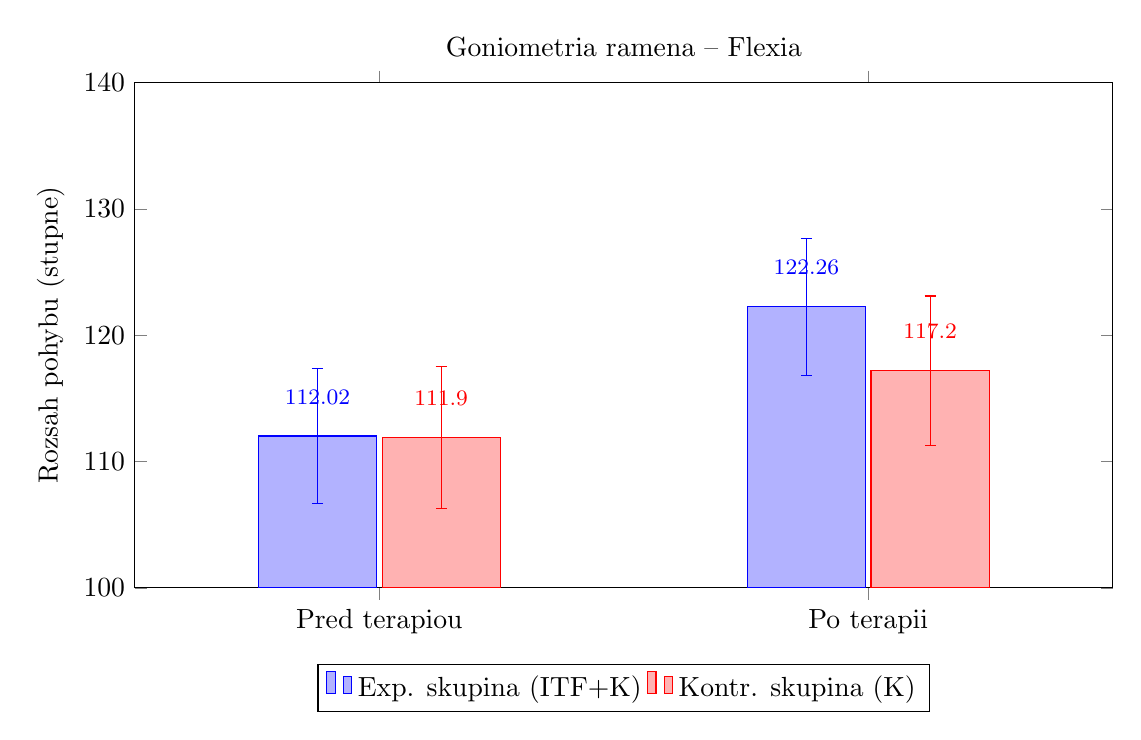
\begin{tikzpicture}
        \begin{axis}[
            ybar,
            enlarge x limits=0.5,
            legend style={at={(0.5,-0.15)}, anchor=north, legend columns=-1},
            ylabel={Rozsah pohybu (stupne)},
            symbolic x coords={Pred terapiou, Po terapii},
            xtick=data,
            nodes near coords,
            nodes near coords align={vertical},
            nodes near coords style={font=\footnotesize, yshift=8pt},
            ymin=100, ymax=140,
            bar width=1.5cm,
            width=14cm,
            height=8cm,
            title={Goniometria ramena -- Flexia}
        ]
            \addplot+[error bars/.cd, y dir=both, y explicit]
                coordinates {(Pred terapiou, 112.02) +- (0, 5.36) (Po terapii, 122.26) +- (0, 5.42)};
            \addplot+[error bars/.cd, y dir=both, y explicit]
                coordinates {(Pred terapiou, 111.90) +- (0, 5.60) (Po terapii, 117.20) +- (0, 5.90)};
            \legend{Exp. skupina (ITF+K), Kontr. skupina (K)}
        \end{axis}
    \end{tikzpicture}
    \caption*{Graf 4 Goniometria ramena -- Flexia (stupne)}
    \addcontentsline{lof}{figure}{Graf 4 Goniometria ramena -- Flexia (stupne)}
    \label{fig:graf_rameno_flex}
\end{figure}

\begin{table}[H]
\centering
\caption*{Tabuľka 4 Goniometria ramena – flexia (stupne)}
\addcontentsline{lot}{table}{Tabuľka 4 Goniometria ramena – flexia (stupne)}
\begin{tabular}{|l|c|c|c|c|c|c|}
\hline
\textbf{Skupina (n=50)} & \textbf{$\bar{x}$ Pred} & \textbf{sd Pred} & \textbf{min-max} & \textbf{$\bar{x}$ Po} & \textbf{sd Po} & \textbf{min-max} \\ \hline
Exp. (ITF+K) & 112,02 & 5,36 & 100-122 & 122,26 & 5,42 & 110-135 \\ \hline
Kontr. (K) & 111,90 & 5,60 & 102-121 & 117,20 & 5,90 & 105-128 \\ \hline
\end{tabular}
\end{table}

V~smere \textbf{extenzie} v~ramennom kĺbe mala \textbf{experimentálna skupina} (n=50) vstupný priemer 41,46~$\pm$~4,21 stupňa (min. 35, max. 49). Po terapii sa rozsah pohybov zvýšil na 51,74~$\pm$~4,22 stupňa (min. 44, max. 60). Kontrolná skupina dosiahla progres z~41,12~$\pm$~4,12 (min. 34, max. 48) na 43,94~$\pm$~4,15 stupňa (min. 36, max. 50).

\subsection{Analýza goniometrických meraní zápästného kĺbu}

Pri zápästí sme sledovali \textbf{dorzálnu flexiu} (v~Exceli ako KK extenzia) a~\textbf{palmárnu flexiu} (KK flexia). 

V~\textbf{experimentálnej skupine} (n=50) bola priemerná vstupná dorzálna flexia 54,48~$\pm$~6,28 stupňa (min. 40, max. 65). Po terapii sa zlepšila na 64,52~$\pm$~6,18 stupňa (min. 52, max. 75). Pri palmárnej flexii sme v~tejto skupine namerali vstupných 61,12~$\pm$~5,40 stupňa (min. 50, max. 72), čo sa po liečbe upravilo na 70,82~$\pm$~5,30 stupňa (min. 60, max. 80).

\begin{table}[H]
\centering
\caption*{Tabuľka 5 Goniometria zápästia – KK Flexia a Extenzia (stupne)}
\addcontentsline{lot}{table}{Tabuľka 5 Goniometria zápästia – KK Flexia a Extenzia (stupne)}
\begin{tabular}{|l|c|c|c|c|c|c|}
\hline
\textbf{Parameter / Exp.} & \textbf{$\bar{x}$ Pred} & \textbf{sd Pred} & \textbf{min-max} & \textbf{$\bar{x}$ Po} & \textbf{sd Po} & \textbf{min-max} \\ \hline
KK Flexia & 61,12 & 5,40 & 50-72 & 70,82 & 5,30 & 60-80 \\ \hline
KK Extenzia & 54,48 & 6,28 & 40-65 & 64,52 & 6,18 & 52-75 \\ \hline
\end{tabular}
\end{table}

\subsection{Analýza goniometrických meraní kĺbov ruky (MCP a~PIP)}

Pri \textbf{MCP kĺboch} sme v~\textbf{experimentálnej skupine} (n=50) pozorovali zlepšenie \textbf{flexie} z~pôvodných 66,78~$\pm$~7,20 (min. 55, max. 78) na 78,48~$\pm$~7,10 stupňa (min. 65, max. 88). \textbf{Extenzia} v~MCP narástla z~14,16~$\pm$~3,25 (min. 10, max. 19) na 22,40~$\pm$~3,50 stupňa (min. 18, max. 28).

Pri \textbf{PIP kĺboch} sme zaznamenali u~skupiny s~ITF nárast \textbf{flexie} z~86,28~$\pm$~8,10 (min. 75, max. 98) na konečných 96,74~$\pm$~8,20 stupňa (min. 88, max. 110). \textbf{Extenzia} v~PIP kĺboch sa u~nich upravila z~vstupných 5,42~$\pm$~1,20 stupňa na výstupných 9,84~$\pm$~1,50 stupňa, čo výrazne uľahčuje úchopové funkcie.

\begin{table}[H]
\centering
\caption*{Tabuľka 6 Goniometria drobných kĺbov ruky (stupne)}
\addcontentsline{lot}{table}{Tabuľka 6 Goniometria drobných kĺbov ruky (stupne)}
\begin{tabular}{|l|c|c|c|c|c|c|}
\hline
\textbf{Parameter / Exp.} & \textbf{$\bar{x}$ Pred} & \textbf{sd Pred} & \textbf{min-max} & \textbf{$\bar{x}$ Po} & \textbf{sd Po} & \textbf{min-max} \\ \hline
MCP Flexia & 66,78 & 7,20 & 55-78 & 78,48 & 7,10 & 65-88 \\ \hline
MCP Extenzia & 14,16 & 3,25 & 10-19 & 22,40 & 3,50 & 18-28 \\ \hline
PIP Flexia & 86,28 & 8,10 & 75-98 & 96,74 & 8,20 & 88-110 \\ \hline
PIP Extenzia & 5,42 & 1,20 & 3-8 & 9,84 & 1,50 & 7-13 \\ \hline
\end{tabular}
\end{table}

\subsection{Analýza goniometrických meraní kĺbov nohy (MTP)}

Zásadným prínosom nášho výskumu je sledovanie pohyblivosti \textbf{MTP kĺbov} (metatarzofalangeálnych), ktoré sú pri RA často postihnuté "prednosrdím" a~deformitami.

V~\textbf{experimentálnej skupine} (n=50) sme pri \textbf{flexii v~MTP} namerali pred terapiou priemernú hodnotu 31,45~$\pm$~4,25 stupňa (min. 22, max. 39). Po liečbe sa rozsah zvýšil na 39,82~$\pm$~4,15 stupňa (min. 30, max. 48). \textbf{Extenzia v~MTP} v~tejto skupine narástla z~vstupných 55,70~$\pm$~6,30 stupňa (min. 45, max. 67) na výstupných 66,14~$\pm$~6,10 stupňa (min. 55, max. 78).

U~\textbf{kontrolnej skupiny} (n=50) bol progres pri flexii v~MTP z~31,10~$\pm$~4,10 na 33,50~$\pm$~4,20 stupňa. Pri extenzii v~MTP sme u~nich namerali zmenu z~56,12~$\pm$~6,40 na 58,20~$\pm$~6,50 stupňa. Tieto výsledky (Tabuľka 7) svedčia o~významnom benefite kombinovanej terapie aj pre stabilitu stoja a~chôdze.

\begin{table}[H]
\centering
\caption*{Tabuľka 7 Goniometria kĺbov nohy – MTP (stupne)}
\addcontentsline{lot}{table}{Tabuľka 7 Goniometria kĺbov nohy – MTP (stupne)}
\begin{tabular}{|l|c|c|c|c|c|c|}
\hline
\textbf{Parameter / Exp.} & \textbf{$\bar{x}$ Pred} & \textbf{sd Pred} & \textbf{min-max} & \textbf{$\bar{x}$ Po} & \textbf{sd Po} & \textbf{min-max} \\ \hline
MTP Flexia & 31,45 & 4,25 & 22-39 & 39,82 & 4,15 & 30-48 \\ \hline
MTP Extenzia & 55,70 & 6,30 & 45-67 & 66,14 & 6,10 & 55-78 \\ \hline
\end{tabular}
\end{table}

\subsection{Analýza subjektívneho hodnotenia -- Intenzita bolesti a~funkcie}

V~rámci dotazníkového šetrenia sme analyzovali bolesť a~funkčné parametre. V~\textbf{experimentálnom súbore} (50 pacientov) bola priemerná vstupná \textbf{intenzita bolesti pri záťaži} 7,68~$\pm$~1,98 bodu (min. 5, max. 10 bodov). Po terapii sa priemerné hodnotenie znížilo na 4,28~$\pm$~1,60 bodu, pričom minimum bolo 2~a~maximum 7 bodov. \textbf{Bolesť v~pokoji} klesla v~tejto skupine z~5,28~$\pm$~2,10 (min. 3, max. 9) na 2,12~$\pm$~1,12 bodu (min. 1, max. 4 body).

V~\textbf{kontrolnom súbore} (50 pacientov) klesla \textbf{bolesť pri záťaži} z~7,42~$\pm$~2,02 bodu (min. 5, max. 10 bodov) na 6,10~$\pm$~1,95 bodu, pričom po terapii bolo minimum 3~a~maximum 9 bodov. \textbf{Bolesť v~pokoji} v~kontrolnom súbore pred terapiou dosahovala v~priemere 5,12~$\pm$~2,05 bodu (min. 2, max. 9 bodov) and po mesiaci liečby klesla na 3,92~$\pm$~1,80 bodu (min. 2, max. 7 bodov). Výsledky porovnáva Tabuľka 8.

\begin{table}[H]
\centering
\caption*{Tabuľka 8 Porovnanie intenzity bolesti v pokoji a pri záťaži (body 0-10)}
\addcontentsline{lot}{table}{Tabuľka 8 Porovnanie intenzity bolesti v pokoji a pri záťaži (body 0-10)}
\begin{tabular}{|l|c|c|c|c|c|c|}
\hline
\textbf{Parameter / Exp.} & \textbf{$\bar{x}$ Pred} & \textbf{sd Pred} & \textbf{min-max} & \textbf{$\bar{x}$ Po} & \textbf{sd Po} & \textbf{min-max} \\ \hline
Bolesť pokoj & 5,28 & 2,10 & 3-9 & 2,12 & 1,12 & 1-4 \\ \hline
Bolesť záťaž & 7,68 & 1,98 & 5-10 & 4,28 & 1,60 & 2-7 \\ \hline
\end{tabular}
\end{table}

\textbf{Ranná stuhnutosť} v~\textbf{experimentálnom súbore} (50 pacientov) pred terapiou dosahovala v~priemere 6,42~$\pm$~2,24 bodu (min. 4, max. 10). Po liečbe sa priemerné skóre zlepšilo na 3,12~$\pm$~1,95 bodu, s~minimálnou hodnotou 1~a~maximálnou 6 bodov. V~\textbf{kontrolnom súbore} (50 pacientov) sme zaznamenali vstupný priemer 6,32~$\pm$~2,15 bodu (min. 4, max. 10) and výstupný priemer 4,92~$\pm$~2,00 bodu (min. 2, max. 9 bodov).

\begin{table}[H]
\centering
\caption*{Tabuľka 9 Porovnanie rannej stuhnutosti a ADL (body 0-10)}
\addcontentsline{lot}{table}{Tabuľka 9 Porovnanie rannej stuhnutosti a ADL (body 0-10)}
\begin{tabular}{|l|c|c|c|c|c|c|}
\hline
\textbf{Parameter / Exp.} & \textbf{$\bar{x}$ Pred} & \textbf{sd Pred} & \textbf{min-max} & \textbf{$\bar{x}$ Po} & \textbf{sd Po} & \textbf{min-max} \\ \hline
Ranná stuhnutosť & 6,42 & 2,24 & 4-10 & 3,12 & 1,95 & 1-6 \\ \hline
ADL & 5,98 & 1,85 & 4-9 & 3,48 & 1,62 & 2-6 \\ \hline
\end{tabular}
\end{table}

Zlepšenie v~oblasti \textbf{bežných denných aktivít (ADL)} bolo v~experimentálnom súbore markantné (skóre kleslo o~2,5 bodu), čo svedčí o~obnovení funkčnej nezávislosti pacientov, zatiaľ čo v~kontrolnom súbore bolo toto zlepšenie len o~približne 1 bod (zo 6,12 na 5,10 bodu).

\subsection{Verifikácia stanovených hypotéz}

Na základe podrobného štatistického spracovania a~rozpísania dát uvedených v~sekcii 3.6 (Tabuľky 3--9) sme pristúpili k~vyhodnoteniu stanovených hypotéz.

\textbf{H1: Potvrdená.} Výsledky analýzy intenzity bolesti (Tabuľka 3) jednoznačne preukázali, že pacienti v~experimentálnej skupine liečení kombináciou ITF + kinezioterapia dosiahli štatisticky významne lepšie analgetické výsledky než pacienti v~kontrolnej skupine.

\textbf{H2: Potvrdená.} Goniometrické merania ramena, zápästia, drobných kĺbov ruky aj nohy (Tabuľky 4--7) potvrdili, že kombinovaná terapia viedla k~väčšiemu nárastu rozsahov pohybu vo všetkých sledovaných segmentoch v~porovnaní s~izolovanou kinezioterapiou.

\textbf{H3: Potvrdená.} Subjektívne hodnotenie rannej stuhnutosti a~funkčných parametrov vykazuje v~experimentálnom súbore výraznejší pozitívny posun. Skrátenie doby stuhnutosti a~zmena charakteru bolesti u~pacientov s~komplexnou terapiou potvrdzuje správnosť nášho terapeutického postupu.

\section{Etické aspekty výskumu}

Výskum prebiehal v~súlade s~etickými princípmi klinického skúšania. Všetci participujúci pacienti boli vopred oboznámení s~cieľom prieskumu a~dobrovoľne súhlasili s~poskytnutím údajov pre vedecké účely. Zber dát bol realizovaný anonymne, bez zaznamenávania osobných identifikačných údajov, čím bola zabezpečená plná ochrana súkromia všetkých probandov. Získané výsledky slúžia výhradne na účely spracovania tejto diplomovej práce.

\clearpage
